\documentclass[11pt,]{article}
\usepackage[left=1in,top=1in,right=1in,bottom=1in]{geometry}
\newcommand*{\authorfont}{\fontfamily{phv}\selectfont}
\usepackage[]{mathpazo}


  \usepackage[T1]{fontenc}
  \usepackage[utf8]{inputenc}




\usepackage{abstract}
\renewcommand{\abstractname}{}    % clear the title
\renewcommand{\absnamepos}{empty} % originally center

\renewenvironment{abstract}
 {{%
    \setlength{\leftmargin}{0mm}
    \setlength{\rightmargin}{\leftmargin}%
  }%
  \relax}
 {\endlist}

\makeatletter
\def\@maketitle{%
  \newpage
%  \null
%  \vskip 2em%
%  \begin{center}%
  \let \footnote \thanks
    {\fontsize{18}{20}\selectfont\raggedright  \setlength{\parindent}{0pt} \@title \par}%
}
%\fi
\makeatother




\setcounter{secnumdepth}{0}

\usepackage{color}
\usepackage{fancyvrb}
\newcommand{\VerbBar}{|}
\newcommand{\VERB}{\Verb[commandchars=\\\{\}]}
\DefineVerbatimEnvironment{Highlighting}{Verbatim}{commandchars=\\\{\}}
% Add ',fontsize=\small' for more characters per line
\usepackage{framed}
\definecolor{shadecolor}{RGB}{248,248,248}
\newenvironment{Shaded}{\begin{snugshade}}{\end{snugshade}}
\newcommand{\AlertTok}[1]{\textcolor[rgb]{0.94,0.16,0.16}{#1}}
\newcommand{\AnnotationTok}[1]{\textcolor[rgb]{0.56,0.35,0.01}{\textbf{\textit{#1}}}}
\newcommand{\AttributeTok}[1]{\textcolor[rgb]{0.77,0.63,0.00}{#1}}
\newcommand{\BaseNTok}[1]{\textcolor[rgb]{0.00,0.00,0.81}{#1}}
\newcommand{\BuiltInTok}[1]{#1}
\newcommand{\CharTok}[1]{\textcolor[rgb]{0.31,0.60,0.02}{#1}}
\newcommand{\CommentTok}[1]{\textcolor[rgb]{0.56,0.35,0.01}{\textit{#1}}}
\newcommand{\CommentVarTok}[1]{\textcolor[rgb]{0.56,0.35,0.01}{\textbf{\textit{#1}}}}
\newcommand{\ConstantTok}[1]{\textcolor[rgb]{0.00,0.00,0.00}{#1}}
\newcommand{\ControlFlowTok}[1]{\textcolor[rgb]{0.13,0.29,0.53}{\textbf{#1}}}
\newcommand{\DataTypeTok}[1]{\textcolor[rgb]{0.13,0.29,0.53}{#1}}
\newcommand{\DecValTok}[1]{\textcolor[rgb]{0.00,0.00,0.81}{#1}}
\newcommand{\DocumentationTok}[1]{\textcolor[rgb]{0.56,0.35,0.01}{\textbf{\textit{#1}}}}
\newcommand{\ErrorTok}[1]{\textcolor[rgb]{0.64,0.00,0.00}{\textbf{#1}}}
\newcommand{\ExtensionTok}[1]{#1}
\newcommand{\FloatTok}[1]{\textcolor[rgb]{0.00,0.00,0.81}{#1}}
\newcommand{\FunctionTok}[1]{\textcolor[rgb]{0.00,0.00,0.00}{#1}}
\newcommand{\ImportTok}[1]{#1}
\newcommand{\InformationTok}[1]{\textcolor[rgb]{0.56,0.35,0.01}{\textbf{\textit{#1}}}}
\newcommand{\KeywordTok}[1]{\textcolor[rgb]{0.13,0.29,0.53}{\textbf{#1}}}
\newcommand{\NormalTok}[1]{#1}
\newcommand{\OperatorTok}[1]{\textcolor[rgb]{0.81,0.36,0.00}{\textbf{#1}}}
\newcommand{\OtherTok}[1]{\textcolor[rgb]{0.56,0.35,0.01}{#1}}
\newcommand{\PreprocessorTok}[1]{\textcolor[rgb]{0.56,0.35,0.01}{\textit{#1}}}
\newcommand{\RegionMarkerTok}[1]{#1}
\newcommand{\SpecialCharTok}[1]{\textcolor[rgb]{0.00,0.00,0.00}{#1}}
\newcommand{\SpecialStringTok}[1]{\textcolor[rgb]{0.31,0.60,0.02}{#1}}
\newcommand{\StringTok}[1]{\textcolor[rgb]{0.31,0.60,0.02}{#1}}
\newcommand{\VariableTok}[1]{\textcolor[rgb]{0.00,0.00,0.00}{#1}}
\newcommand{\VerbatimStringTok}[1]{\textcolor[rgb]{0.31,0.60,0.02}{#1}}
\newcommand{\WarningTok}[1]{\textcolor[rgb]{0.56,0.35,0.01}{\textbf{\textit{#1}}}}

\usepackage{graphicx,grffile}
\makeatletter
\def\maxwidth{\ifdim\Gin@nat@width>\linewidth\linewidth\else\Gin@nat@width\fi}
\def\maxheight{\ifdim\Gin@nat@height>\textheight\textheight\else\Gin@nat@height\fi}
\makeatother
% Scale images if necessary, so that they will not overflow the page
% margins by default, and it is still possible to overwrite the defaults
% using explicit options in \includegraphics[width, height, ...]{}
\setkeys{Gin}{width=\maxwidth,height=\maxheight,keepaspectratio}


\title{Patient's age prediction based on medical diagnosis of teeth
maturity \thanks{We would like to thanks the doctors who delivered their
experienced assesment of teeth maturity as well as our teacher who
provided us the data to work with.}  }
 



\author{\Large De La Torre
Camilo\vspace{0.05in} \newline\normalsize\emph{Universite Toulouse 1
Capitole}   \and \Large Campan
Alexis\vspace{0.05in} \newline\normalsize\emph{Universite Toulouse 1
Capitole}  }


\date{}

\usepackage{titlesec}

\titleformat*{\section}{\normalsize\bfseries}
\titleformat*{\subsection}{\normalsize\itshape}
\titleformat*{\subsubsection}{\normalsize\itshape}
\titleformat*{\paragraph}{\normalsize\itshape}
\titleformat*{\subparagraph}{\normalsize\itshape}



\usepackage{biblatex}

\addbibresource{master.bib}


\newtheorem{hypothesis}{Hypothesis}
\usepackage{setspace}


% set default figure placement to htbp
\makeatletter
\def\fps@figure{htbp}
\makeatother


% move the hyperref stuff down here, after header-includes, to allow for - \usepackage{hyperref}

\makeatletter
\@ifpackageloaded{hyperref}{}{%
\ifxetex
  \PassOptionsToPackage{hyphens}{url}\usepackage[setpagesize=false, % page size defined by xetex
              unicode=false, % unicode breaks when used with xetex
              xetex]{hyperref}
\else
  \PassOptionsToPackage{hyphens}{url}\usepackage[draft,unicode=true]{hyperref}
\fi
}

\@ifpackageloaded{color}{
    \PassOptionsToPackage{usenames,dvipsnames}{color}
}{%
    \usepackage[usenames,dvipsnames]{color}
}
\makeatother
\hypersetup{breaklinks=true,
            bookmarks=true,
            pdfauthor={De La Torre Camilo (Universite Toulouse 1
Capitole) and Campan Alexis (Universite Toulouse 1 Capitole)},
             pdfkeywords = {Teeth, Age, Regression, Machine Learning,
GBRT},  
            pdftitle={Patient's age prediction based on medical
diagnosis of teeth maturity},
            colorlinks=true,
            citecolor=blue,
            urlcolor=blue,
            linkcolor=magenta,
            pdfborder={0 0 0}}
\urlstyle{same}  % don't use monospace font for urls

% Add an option for endnotes. -----


% add tightlist ----------
\providecommand{\tightlist}{%
\setlength{\itemsep}{0pt}\setlength{\parskip}{0pt}}

% add some other packages ----------

% \usepackage{multicol}
% This should regulate where figures float
% See: https://tex.stackexchange.com/questions/2275/keeping-tables-figures-close-to-where-they-are-mentioned
\usepackage[section]{placeins}


\begin{document}
	
% \pagenumbering{arabic}% resets `page` counter to 1 
%    

% \maketitle

{% \usefont{T1}{pnc}{m}{n}
\setlength{\parindent}{0pt}
\thispagestyle{plain}
{\fontsize{18}{20}\selectfont\raggedright 
\maketitle  % title \par  

}

{
   \vskip 13.5pt\relax \normalsize\fontsize{11}{12} 
\textbf{\authorfont De La Torre
Camilo} \hskip 15pt \emph{\small Universite Toulouse 1
Capitole}   \par \textbf{\authorfont Campan
Alexis} \hskip 15pt \emph{\small Universite Toulouse 1 Capitole}   

}

}








\begin{abstract}

    \hbox{\vrule height .2pt width 39.14pc}

    \vskip 8.5pt % \small 

\noindent Our study involves patient's age prediction based on teeth
maturity that is assesed by doctors. Teeth are characterised by several
levels of maturity (going from A to H), data is often incomplete and for
some patients, teeth can't be evaluated because the patient does not
have them yet. After several attempts to mitigate the incompleteness of
our records, we obtained a very low Mean Absolute Error of 0.9 years in
predicting unseen data. The model that best generalized to unseen
records was a tuned GBRT (Gradient Boosting Regression Tree). Lastly, we
also analyse the importance of different teeth maturities and
interestingly discovered that not all teeth have the same predictive
power on patient's age.


\vskip 8.5pt \noindent \emph{Keywords}: Teeth, Age, Regression, Machine
Learning, GBRT \par

    \hbox{\vrule height .2pt width 39.14pc}



\end{abstract}


\vskip -8.5pt


 % removetitleabstract

\noindent  

\hypertarget{introduction}{%
\section{Introduction}\label{introduction}}

The data we study explores teeth maturity of several individuals,
specifically, we analysed 2847 records. By teeth maturity we mean that
each tooth's condition is analysed by a doctor and classed on one of the
possible maturity levels (going from A to H, A being the least mature,
and H being the most mature). A total of 8 teeth are analysed by
doctors, these involve : two incisors teeth, one canine tooth, two
premolar teeth, finally, three molar teeth. In addition to teeth
maturity indices, we also know the patient's sex, age and medical ID.

\hypertarget{incompleteness-of-the-data}{%
\section{Incompleteness of the data}\label{incompleteness-of-the-data}}

The data at hand is not complete: out of our 2847 records, for 1436
records at least a tooth score is missing (50\% of the data). Moreover,
not all teeth are equally misrepresented, as we might expect, molar
teeth scores are less likely to be present in our records because
several patients do not have them yet. In addition, because of multiple
reasons, is it possible that a patient of a given age lost or had
removed one or several teeth, this, we think, complicates missing values
interpretation because several causes, unrelated to age, can affect it.

Figure X shows missing values per column in our data, moreover, it shows
the interaction between missing values across columns.

We observe that our dependent variable, patient's age, is always
complete. We also note that the last molar has a very high percentage of
missing values. Besides the last molar (M3), another two teeth have over
10\% of missing values (I1 and PM2).

\begin{verbatim}
## Warning: `gather_()` was deprecated in tidyr 1.2.0.
## Please use `gather()` instead.
\end{verbatim}

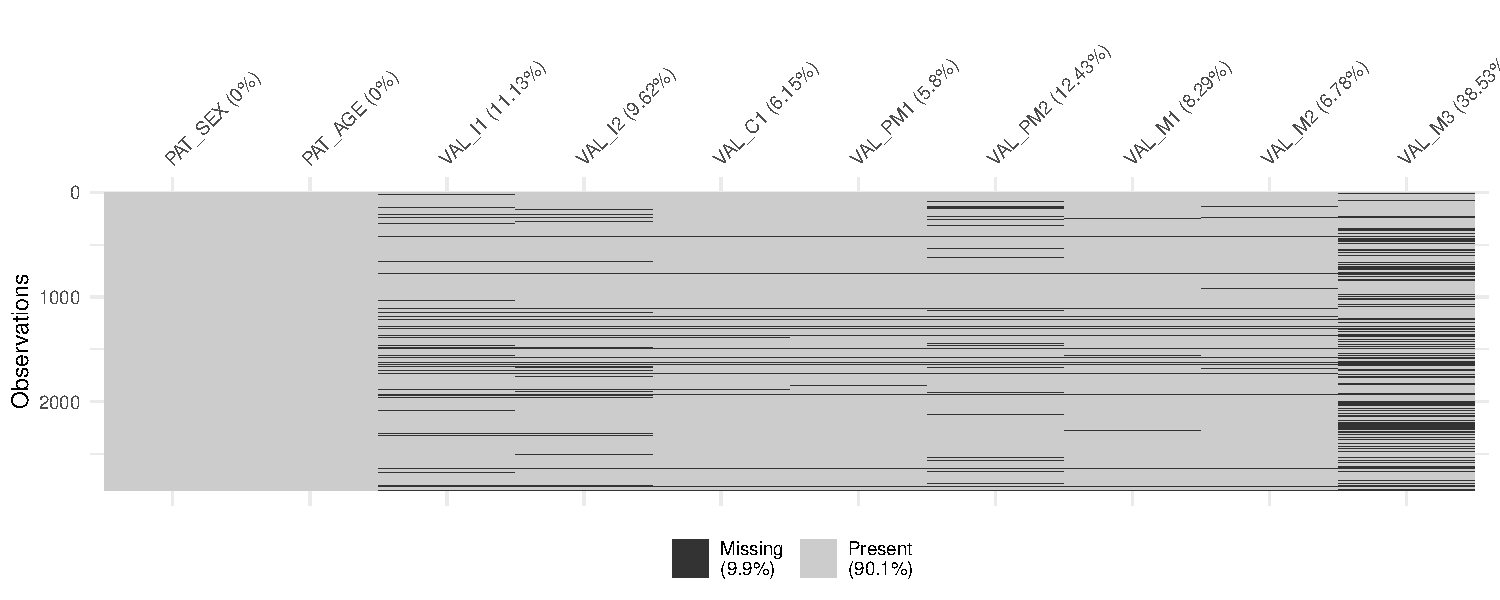
\includegraphics{paper_teeth_files/figure-latex/unnamed-chunk-3-1.pdf}

Nonetheless, because of the first reason of incompleteness we presented
(that teeth grow at different stages in life) we think that imputing
missing values makes sense, our approach is explained when we discuss
about our methodology.

\hypertarget{methodology}{%
\section{Methodology}\label{methodology}}

As predictive power is our main goal, we are interested in finding the
model that minimizes an error score on unseen data. The score we chose
is the Mean Absolute Error defined as
\(mae=(\frac{1}{n})\sum_{i=1}^{n}\left | y_{i} - f(x_{i}) \right |\)
where \(f(x_{i})\) is our predicted age.

To do so, we adopt a classical random split of our data to avoid any
data leakage and test model generalization. For algorithms that do not
make a validation set right out the bat, i.e.~\emph{XGBoost}, we make it
ourselves to ensure that we do not overfit our model on test data
because of Early Stopping and other techniques.

\hypertarget{ordinal-encoding}{%
\subsection{Ordinal encoding}\label{ordinal-encoding}}

Teeth maturity comes in a mixture of numbers and letters levels.
Maturity scores ranges from 0, 1, A,\ldots, H, 0 being the least mature
and H being the most mature. Several algorithms do not work with ordinal
data or perform poorly after one hot encoding of such data.

In order to compare algorithms but also to facilitate convergence on
some algorithms we adopt the strategy of ordinal encoding. That is, we
assign an integer value to each categorical level. The transformation is
monotonic for the purpose of keeping the order of teeth maturity scores.

We assume that maturity scores are based on a linear scale, in other
words, the difference between A and B is of the same magnitude as the
difference between G and H.

\hypertarget{handling-missing-values}{%
\subsection{Handling missing values}\label{handling-missing-values}}

\hypertarget{removing-very-incomplete-data}{%
\subsubsection{Removing very incomplete
data}\label{removing-very-incomplete-data}}

As discussed before, several samples of the data contain missing values.
Figure X showed that for several patients, multiple teeth scores where
missing, i.e.~some samples presented a continuous black line, indicating
that for all teeth, the maturity scores are not available. Because of
this observation, we decided to exclude some samples from the training
data in order to prevent the imputation technique, discussed below, to
base its neighboring on an insufficient subset of columns.

Specifically, we removed samples in the training set for which
information about 7, out of 8, teeth is missing. That was the case for
108 samples in the training set, reducing its size from 2135
observations to 2027 observations.

\hypertarget{k-nearest-neighbors-imputation}{%
\subsubsection{K Nearest Neighbors
imputation}\label{k-nearest-neighbors-imputation}}

We believe that, in general, patients of similar age have similar teeth
maturities, hence, we are convinced that for our prediction task,
samples that are alike will tend to have the same age. Therefore, if
tooth information is missing from a sample, we believe that it could be
estimated by looking at analogous samples existing in the training data.
This motivates us to use an imputing algorithm that performs some
multivariate estimation of missing values using complete observations.

We performed K Nearest Neighbors imputation on the missing values in the
training set and testing set. We set the vicinity used for imputation to
40 neighbors, these are weighted by euclidean distance.

Because we believe that the missingness of a tooth score is informative
about a patient's age, e.g.~wisdom tooth removal, we created a binary
features indicating the presence of missing values for each imputed
column and sample.

\hypertarget{outlier-removal}{%
\subsection{Outlier removal}\label{outlier-removal}}

After all these steps, our last process before training is to remove the
outliers. Removing outliers consist of exclude unusual values and so
reduce the variability in our data. We have tried several techniques for
detect these outliers: - PCA: we fit\_transform our data and then we
calculate the MSE score for each point in order to drop the 10\% lower
(we have tested 10\% upper and 5\%-5\% but lower values was the best to
remove). - Isolation Forest: this algorithm is based on tree algorithms
it calculate an anomalie score for each point, the easier it is to
isolate the data, the more likely it is that the data is an anomaly.
After performance comparisons we kept the Isolation Forest to remove the
outliers. Remove outliers is one of our most important techniques of
preprocessing to reduce our mean absolute error.

\hypertarget{model-developement}{%
\section{Model developement}\label{model-developement}}

\hypertarget{baseline-results-on-several-algorithms}{%
\subsection{Baseline results on several
algorithms}\label{baseline-results-on-several-algorithms}}

As stated before, our main goal is finding the optimum predictive power.
To do so, we tried several algorithms on the processed data,
i.e.~following the treatment described before.

We report the scores obtained by the following models: Linear
regression, Random Forest, Lasso regression and Elastic regression. All
data sets are scored, that is, the train, validation and test sets. The
models where not \emph{fine tuned} because we were mostly interested in
defining baselines score to improve upon.

In addition, we performed k-fold (k=10) cross validation for each
algorithm to improve our training \emph{mae} estimate. The results of
such cross validation strategy are shown in Figure X:

\begin{Shaded}
\begin{Highlighting}[]
\FunctionTok{autoplot}\NormalTok{(fit\_rs)}
\end{Highlighting}
\end{Shaded}

\includegraphics{paper_teeth_files/figure-latex/autplot-1.pdf}

Table X shows all mean absolute error scores on all data sets from all
models.

\begin{Shaded}
\begin{Highlighting}[]
\FunctionTok{print}\NormalTok{(results)}
\end{Highlighting}
\end{Shaded}

\begin{verbatim}
## # A tibble: 3 x 6
##   data       lm    rf lasso elastic   knn
##   <chr>   <dbl> <dbl> <dbl>   <dbl> <dbl>
## 1 X_train  1.46  1.02  1.46    1.46  1.01
## 2 X_val    1.53  1.12  1.53    1.53  1.44
## 3 X_test   1.55  1.24  1.55    1.55  1.47
\end{verbatim}

\hypertarget{results-on-best-tuned-gbrt}{%
\subsection{Results on best tuned
GBRT}\label{results-on-best-tuned-gbrt}}

\hypertarget{feature-importances}{%
\section{Feature importances}\label{feature-importances}}

\hypertarget{conclusion}{%
\section{Conclusion}\label{conclusion}}





\newpage
\singlespacing 
\printbibliography[title=References]

\end{document}
